

\documentclass{acm_proc_article-sp}
\usepackage{multicol}
\begin{document}

\title{Cluster Based Content Distribution in VANETs}


\numberofauthors{3} 
\author {
% 1st. author
\alignauthor
Aravindan Balan\\
       \email{aravindan@cs.ucla.edu}     
% 2nd. author
\alignauthor 
Chuchu Wu\\
       \email{wuchuchu@cs.ucla.edu}
% 3rd. author
\alignauthor 
Mario Gerla\\
       \email{gerla@cs.ucla.edu}
       \and
\alignauthor 
University of California Los Angeles\\
}

\maketitle
\begin{abstract}
\vspace{1 mm}
The communication-enabled vehicles are interested in downloading different multimedia contents
from Internet-based servers. This system captures many of the entertainment services with
effective information, such as navigation maps, news reporting service, and software updating, or multimedia content downloading. In this approach both infrastructure-to-vehicle and vehicle-vehicle communication take place. It also demands for better performance due to existing difficulties and challenges including limited RSUs available on the road, expensive and limited 3G/LTE resource, etc. By introducing the idea of peer-to-peer content delivery to vehicular networks, cooperative schemes, such as SPAWN \cite{spawn}, significantly improve the efficiency of content downloading in vehicular networks, where the cooperation among vehicles is essential to establish such systems. Hence, uncooperative behavior of peers can severely degrade the system performance, e.g. some vehicles may avoid downloading original data chunks through 3G network in order to save the cost of 3G connection, and only wait for other peers to share with him, i.e. choose to be a free-rider. On the other hand, if too many nodes connect to the 3G/LTE, the 3G/LTE network may encounter serious congestion, and it would be a waste of network resource if many of them are actually downloading the same content.

In this paper, we have proposed a cluster based content distribution scheme for Vehicular Adhoc Networks. Vehicles with common interests form a cluster and take turns to be the cluster head that directly downloads data packets in multiple rounds, especially multimedia content, from the Internet and share with others in the cluster. Our work is mainly focused on highway scenarios in VANETs as vehicles tend to stick together for a considerable amount of time. We have also proposed a novel technique for cluster head selection and also consider other scenarios where vehicles are selfish. We have also investigated the optimal parameters to use to obtain a proper trade-off between efficiency/congestion of the LTE network versus the Robustness of the system. Finally, we have analysed the results on how the selection of optimal parameters affects the network condition. The functionality of our proposed network is verified using ns-3 and SUMO simulations. 

\end{abstract}

\keywords{Peer-to-Peer, Vehicular ad-hoc Network, Multimedia Content Downloading, Cooperative Content Downloading, Cluster-based Content Downloading}

\begin{figure}
\centering
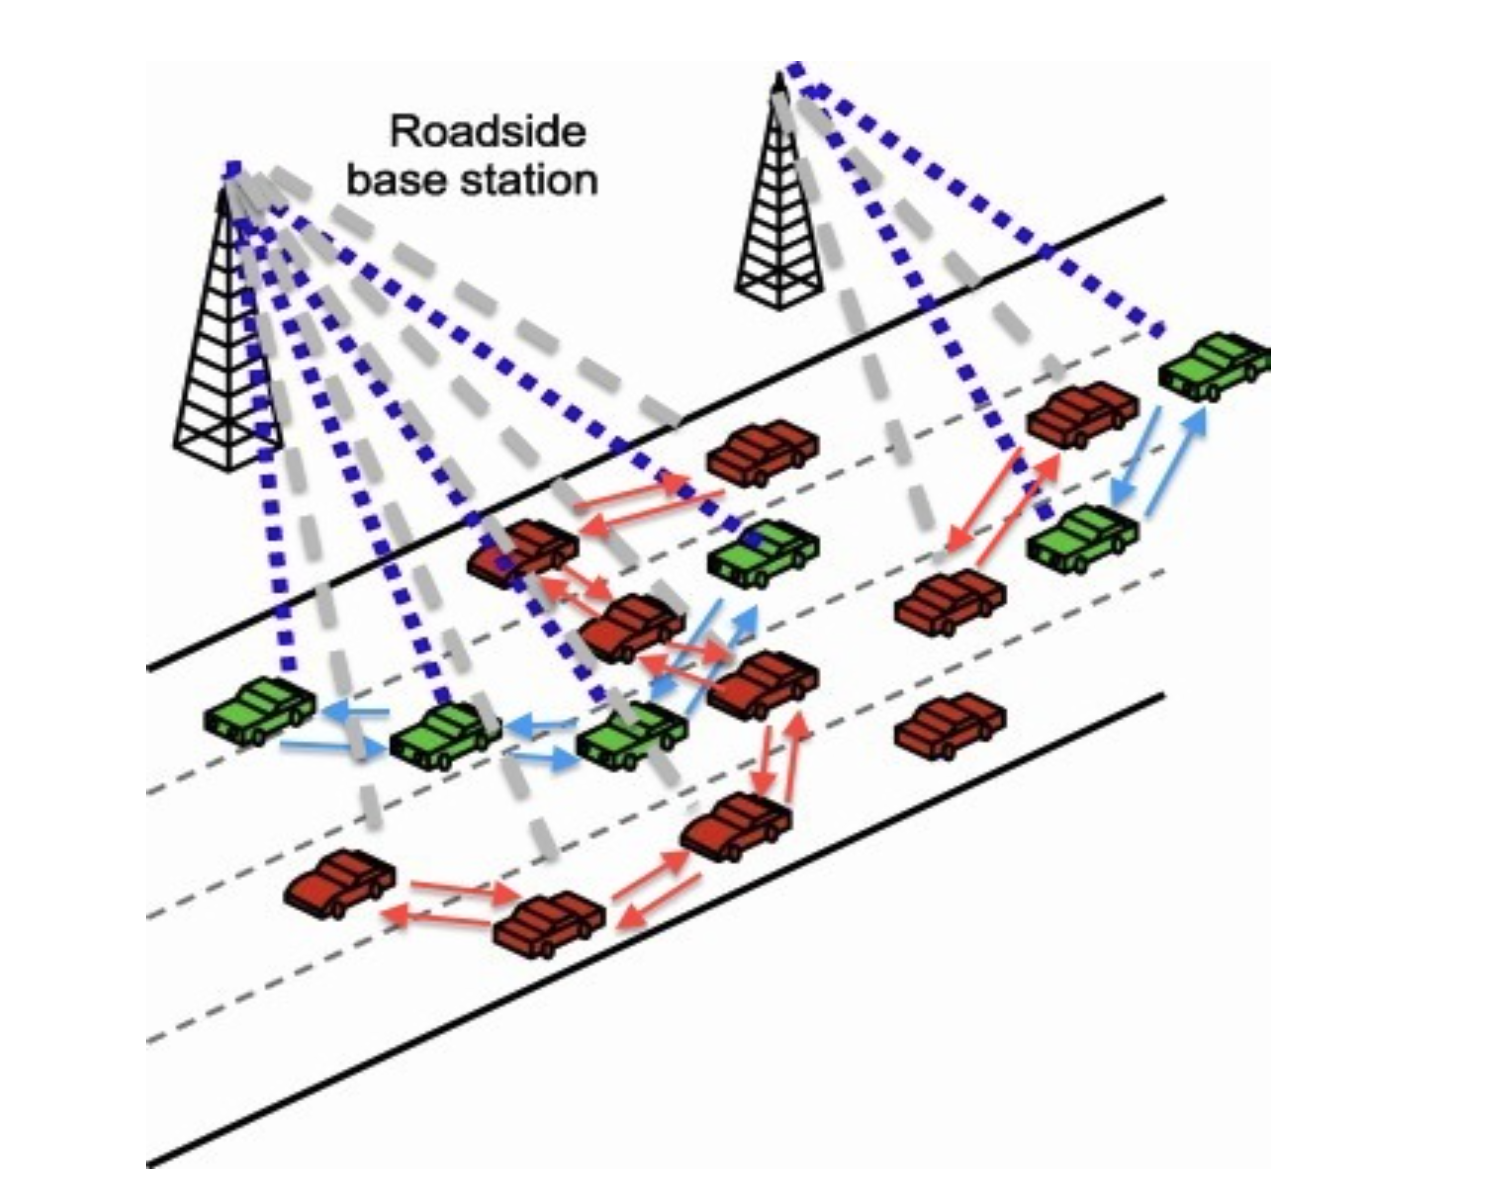
\includegraphics[scale=.33]{working.png} \caption{Cluster Based Content Distribution in VANETs}
\label{working}
\end{figure}

\section{Introduction}
\vspace{1 mm}

Vehicular Ad-hoc Network (VANET) is one of the most emerging areas for the improvement of Intelligent Transportation System (ITS). VANET is a special form of MANET, where Mobile Ad-hoc Network (MANETs) are self-configuring network of mobile nodes connected by wireless links, while, VANET are distributed and self-assembling communication networks. A technology that uses moving vehicles as nodes to create a mobile network is termed as VANET. Here, node movement is restricted by factors like road course, encompassing traffic and traffic regulations. The
primary goal of VANET is to provide road safety and other value added services such as email, audio/video sharing etc.

In the near future, the proliferation of "smart vehicles" is envisaged to become a reality. "Smart vehicles" combine the advantages of both smartphones and laptops: they are as "mobile" as smart phones, i.e. having ubiquitous access to the Internet via 3G/LTE networks, but more powerful in computation and energy supply like laptop computers. Beside safety services, content downloading is expected to be widely popular among drivers and passengers aboard just
like traditional networks. Since the number of road side units is very limited, the time that vehicles can get access to WiFi is very short. So for most of the time, vehicles rely on 3G/LTE to download the contents. However, as data files, such as pictures, audios and videos, are getting larger and larger due to the increasing demands of higher quality of user experience, the 3G/LTE resources, on the contrary, are getting more and more scarce and thus expensive. So the bandwidth assigned to each 3G user is limited which results in long delay of content downloading.

As inter-vehicle communication technology becomes available, cooperative content downloading schemes are proposed to leverage this advantage and bring peer-to-peer overlay network to the vehicular environment. As a typical example, SPAWN \cite{spawn} is a peer-peer content delivery mechanism that utilizes parallel download among a mesh of co-operating peers. Given a very limited amount of RSUs, most of the time, vehicles with common content interest download pieces/chunks of data from the Internet through cellular base stations and share with each other in adhoc mode, as shown in Figure \ref{working}. Such cooperative downloading scheme significantly improve the efficiency of content downloading and shorten the delay.

\section{Related Work}
\vspace{1 mm}

Most existing approaches that improve the efficiency of content downloading in vehicular networks, such as \cite{urban}, \cite{symbol}, \cite{cost}, \cite{indoor}, \cite{opti}, \cite{ondemand}, \cite{datadissem}, \cite{globecom}, rely on the cooperation among vehicles. However, misbehavior among the vehicle community motivated by selfish intentions of saving 3G/LTE bandwidth or energy can severely interfere the network performance. Hence incentive schemes are necessary to enforce the cooperation among nodes in vehicular networks. Incentive schemes, such as \cite{coalitional}, \cite{coop}, \cite{incentive}, \cite{uncoop}, are proposed to enforce the cooperation of intermediate nodes to forward packets in VANETs. Generally, incentive schemes can be categorized into two types, i.e. credit based schemes and reputation based schemes. Credit based schemes are adopted by \cite{coalitional}, \cite{incentive}, \cite{uncoop} where rewards/credits are allocated/paid to the forwarders. A three-counter scheme was proposed in \cite{coop} where nodes count the number of packets for- warded and the number of packets requested to be forwarded as a way of observing and recording the behavior of neighbor nodes, which is fairly similar to the way reputation schemes work. Table.I summarizes the related work according to the application scenarios, whether they are incentive compatible as well as the type of incentive schemes if adopted.

\begin{figure}
\centering
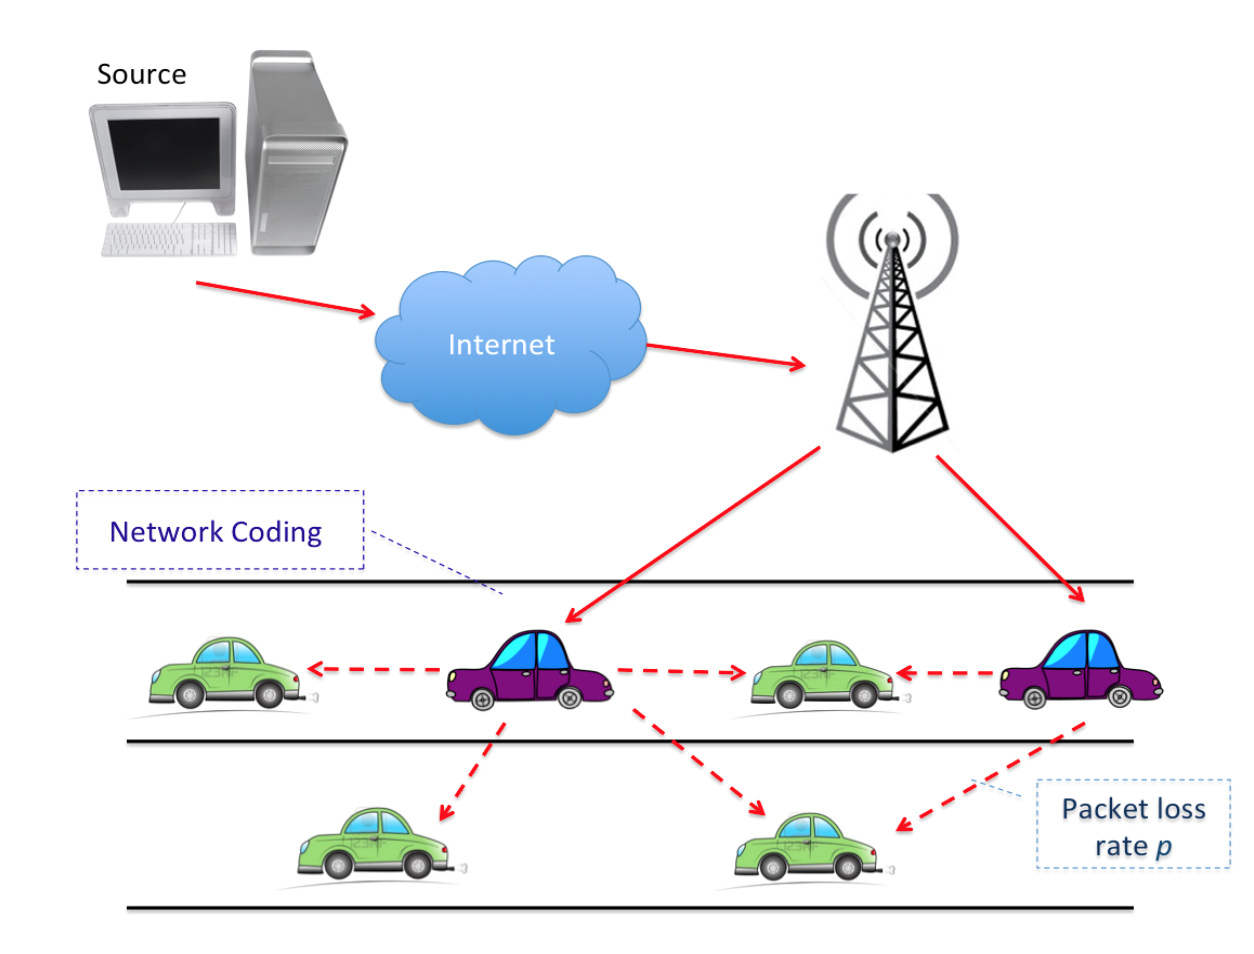
\includegraphics[scale=.30]{design.png} \caption{Overall Design of the System}
\label{design}
\end{figure}

As a matter of fact, the power supply for vehicles is not as a critical issue as for mobile devices, hence nodes in VANETs usually do not have strong intentions to drop the packets from other vehicles in order to save energy. However, 3G/LTE bandwidth is always a scarce resource, no matter for smart phones or smart vehicles. While some smart vehicles download interesting contents from the Internet via 3G/LTE and share with the neighborhood in V2V manner, selfish vehicles may have intentions to be free-riders who benefit from the contributing nodes but refuse to be the contributor itself in order to save its 3G/LTE bandwidth. As to our knowledge, so far there is no incentive scheme designed to enforce the cooperative downloading and maintain fairness for vehicular networks.

\section{ SYSTEM MODEL AND ASSUMPTIONS}
\vspace{1 mm}

\subsection{Network Model}
We consider vehicular networks where vehicles with the same interested contents form a cluster as in Figure \ref{design}. The clusters in the system are managed by a Cluster Manager. The Cluster Manager is responsible for functions like multi-round content delivery, cluster formation, cluster head selection, vehicle churning (vehicles entering and leaving the cluster). All vehicles with the same interested contents form a cluster, as shown in Fig.2. A few cluster heads are selected and they download the original data contents from the Internet source via 3G/LTE network. The cluster heads share their data packets with other vehicles in the cluster, and others may share with each other in a peer-to-peer fashion. 

Our focus was on the Highway scenario of VANET as we can expect lesser node churning and the clusters are intact for a considerable amount of time as compared to Urban scenarios. Having only the cluster head downloading the content, eliminates serious network congestion issues on the network. Also the content is downloaded in multiple rounds and the system uses network coding to eliminate packet losses. We have designed a server-assisting scheduling scheme that both enforces cooperation of vehicles, guarantees sufficiency of cluster head volunteers and efficiency of deciding who is next to be the cluster head. 

\subsection{Working}
The system works in three stages. 

Initially, vehicles express their interest in a particular topic to the Cluster Manager application residing in the RSUs. The cluster manager tries to find a nearby cluster group of same topic of interest or forms a new cluster and add the vehicles either to the respective clusters. 

Following that the cluster manager starts sending the data packets. The data packets are sent in multiple rounds to avoid fragmentation losses due to large packet sizes. The Cluster Manager broadcasts the topic packets to all the masters in the system chosen for that round. Only those masters interested in that particular topic receive the packet . 

The cluster heads then perform network coding (with or without redundancy added) and broadcasts the packet again to all other nodes in the cluster. A vehicle may receive network coded packets from different cluster heads, but still can decode and reconstruct the original content. Also the Cluster manager selects different masters for each round from each cluster thereby ensuring equal participation of all vehicles and avoid selfish vehicles which act as free-riders.  

\begin{figure}
\centering
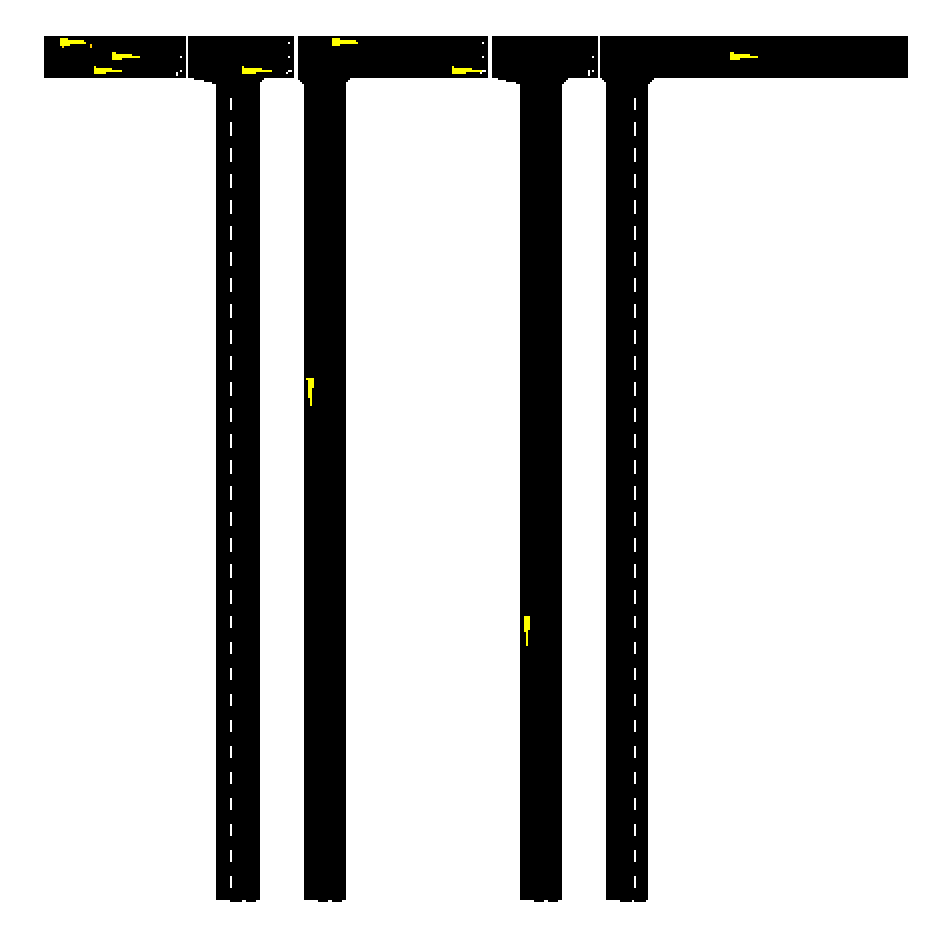
\includegraphics[scale=.40]{sumo.png} \caption{SUMO Highway Layout}
\label{sumo}
\end{figure}

\section{Vanet Simulation using Sumo and NS3}
\vspace{1 mm}

We have simulated the Vanet Highway scenario using SUMO and NS3 \cite{sumons3} as shown in Figure \ref{sumo}.   

\subsection{Simulation of Urban Mobility}

Simulation of Urban Mobility (SUMO) \cite{sumo} is an open source traffic simulation package including net import and demand modelling components. SUMO helps to investigate several research topics e.g. route choice and traffic light algorithm or simulating vehicular communication.the framework is used in different projects to simulate automatic driving or traffic management strategies. Simulations has: space-continuous and time-discrete vehicle movement, different vehicle types, multi-lane streets with lane changing, different right-of-way rules, traffic lights, a fast open GL graphical user interface, manages networks with several edges, fast execution speed, interoperability with other application at run-time, network-wide, edge-based, vehicle-based, and detector-based outputs, supports person-based inter-modal trips, high portability and high interoperability.

We have designed the highway layout with 50 vehicles moving at velocity of 60 mph, 1 stationary RSU, 3 lanes, 4 highway exits. We have mainly focused mainly on the vehicles exiting the system as SUMO is particularly designed for Urban scenarios where vehicles stop before a junction and not for Highway scenarios where vehicles don't stop while entering a highway.

\subsection{NS-3}

NS-3  \cite{ns} is a discrete-event network simulator and a free software which succeeds popular network simulator NS-2.

We have simulated the system using Network Simulator-3 (NS3). We used the trace file generated using SUMO to define the mobility of all the nodes in ns3. So the nodes created in ns3 correspond to the vehicles defined in SUMO. We have also induced a Range Propagation Loss Model with a maximum Range of 100 meters. When a master or slave goes out of range, it is considered to be a packet loss. We use this information to assess the master selection algorithm later.

\section{Results}
\vspace{1 mm}

asdfasfd

\section{Conclusion}
\vspace{1 mm}

sasdfasdfd

\section{Future work}
\vspace{1 mm}

1. choose the optimal cluster head based on the distance from the basestation and the cluster nodes.
2. nodes entering the system.

\begin{thebibliography}{1}

\bibitem{sumons3} Chitraxi Raj,Urvik Upadhayaya ,Twinkle Makwana ,Payal Mahida .Simulation of VANET Using NS-3 and SUMO, Volume 4, Issue 4, Apr 2014.

\bibitem{spawn}A. Nandan, S. Das, G. Pau, M. Gerla, and M. Sanadidi. Co-operative downloading in vehicular ad-hoc wireless networks. In Wireless On- demand Network Systems and Services, 2005. WONS 2005. Second Annual Conference on, pages 32-41, Jan 2005.

\bibitem{sumo}  SUMO - Simulation of Urban MObility {\em http://sumo.sourceforge.net}

\bibitem{ns} The ns-3 network simulator {\em http://www.nsnam.org}

\bibitem{gametheory} Chuchu Wu, Mario Gerla. Game Theoretic Model for Cluster-based Content Distribution in Vehicular Networks, 2014.

\bibitem{coalitional} T. Chen, L. Zhu, F. Wu, and S. Zhong. Stimulating cooperation in vehicular ad hoc networks: A coalitional game theoretic approach. Vehicular Technology, IEEE Transactions on, 60(2):566-579, 2011.

\bibitem{coop} Y. H. Ho, A. H. Ho, G. L. Hamza-Lup, and K. A. Hua. Cooperation enforcement in vehicular networks. In Proceedings of the 2008 Inter- national Conference on Communication Theory, Reliability, and Quality of Service, CTRQ 08, pages 7-12, Washington, DC, USA, 2008. IEEE Computer Society.

\bibitem{urban} H.-C. Jang and T.-Y. Hsu. Urban multi-layered chord for p2p over vehicular network. In Mobile and Wireless Networking (iCOST), 2012 International Conference on Selected Topics in, pages 54-59, 2012.

\bibitem{incentive} F. Li and J. Wu. Frame: An innovative incentive scheme in vehicular networks. In Communications, 2009. ICC 09. IEEE International Conference on, pages 1-6, 2009.

\bibitem{symbol} M. Li, Z. Yang, and W. Lou. Codeon: Cooperative popular content distribution for vehicular networks using symbol level network coding. Selected Areas in Communications, IEEE Journal on, 29(1):223-235, 2011.

\bibitem{cost} T. Luan, L. Cai, J. Chen, X. Shen, and F. Bai. Engineering a distributed infrastructure for large-scale cost-effective content dissemination over urban vehicular networks, 2013.

\bibitem{opti}F.Malandrino,C.Casetti,C.Chiasserini,andM.Fiore.Optimal content downloading in vehicular networks, 2012.

\bibitem{indoor} F.Malandrino, C.Casetti,C.F.Chiasserini, C.Sommer and F.Dressler. Content downloading in vehicular networks: Bringing parked cars into the picture. In Personal Indoor and Mobile Radio Communications (PIMRC), 2012 IEEE 23rd International Symposium on, pages 1534- 1539, 2012.

\bibitem{ondemand} A. Nandan, S. Das, G. Pau, M. Gerla, and M. Sanadidi. Co-operative downloading in vehicular ad-hoc wireless networks. In Wireless On- demand Network Systems and Services, 2005. WONS 2005. Second Annual Conference on, pages 32-41, Jan 2005.

\bibitem{datadissem} T. Wang, L. Song, and Z. Han. Collaborative data dissemination in cognitive vanets with sensing-throughput tradeoff. In Communications in China (ICCC), 2012 1st IEEE International Conference on, pages 41-45, 2012.

\bibitem{uncoop} Z. Wang and C. Chigan. Countermeasure uncooperative behaviors with dynamic trust-token in vanets. In Communications, 2007. ICC 07. IEEE International Conference on, pages 3959-3964, 2007.

\bibitem{globecom} D. Zhang and C.-K. Yeo. A cooperative content distribution system for vehicles. In Global Telecommunications Conference (GLOBECOM 2011), 2011 IEEE, pages 1-6, 2011.

\end{thebibliography}

\end{document}
